\documentclass[a4paper, 11pt]{article}
\usepackage{fullpage} 
\usepackage[margin=1cm]{geometry}
\usepackage{graphicx}
\usepackage{enumitem}
\usepackage{fancyhdr}
\usepackage{multicol}
\usepackage{xhfill}
\usepackage{changepage}

\title{Final Hack: Team Turret}\author{Andy Wong\\Glen Chou\\Lydia Lee}\date{Due: May 5, 2015}
\setlength{\headsep}{1cm}

\begin{document}
\pagestyle{fancy}
\fancyhf{}
\lhead{Team Turret}
\rhead{A. Wong, G. Chou, L. Lee}
\maketitle
\tableofcontents

\newpage
\section{Features}
	\subsection{Rotating Platform}
		The user controls the rotation of the platform via joystick.  Under the hood, a motor with a protected H-bridge turns the platform, while two potentiometers serve as the control system to link the user and platform.
	\subsection{Rubber Band Gun}
		Much like a standard rubber band gun, the firing mechanism is a rotating wheel, except ours is controlled by a button on the joystick that turns a motor.  Initially, the rubber band is held in loaded position by the wheel's rotational inertia.  At button-press, the motor rotates, overcoming the wheel's inertia and firing the rubber band.
\newpage
\section{Schematics}
	\subsection{Table Motor}
	\begin{figure}[!ht]
		\centering
		\vspace{-4cm}
		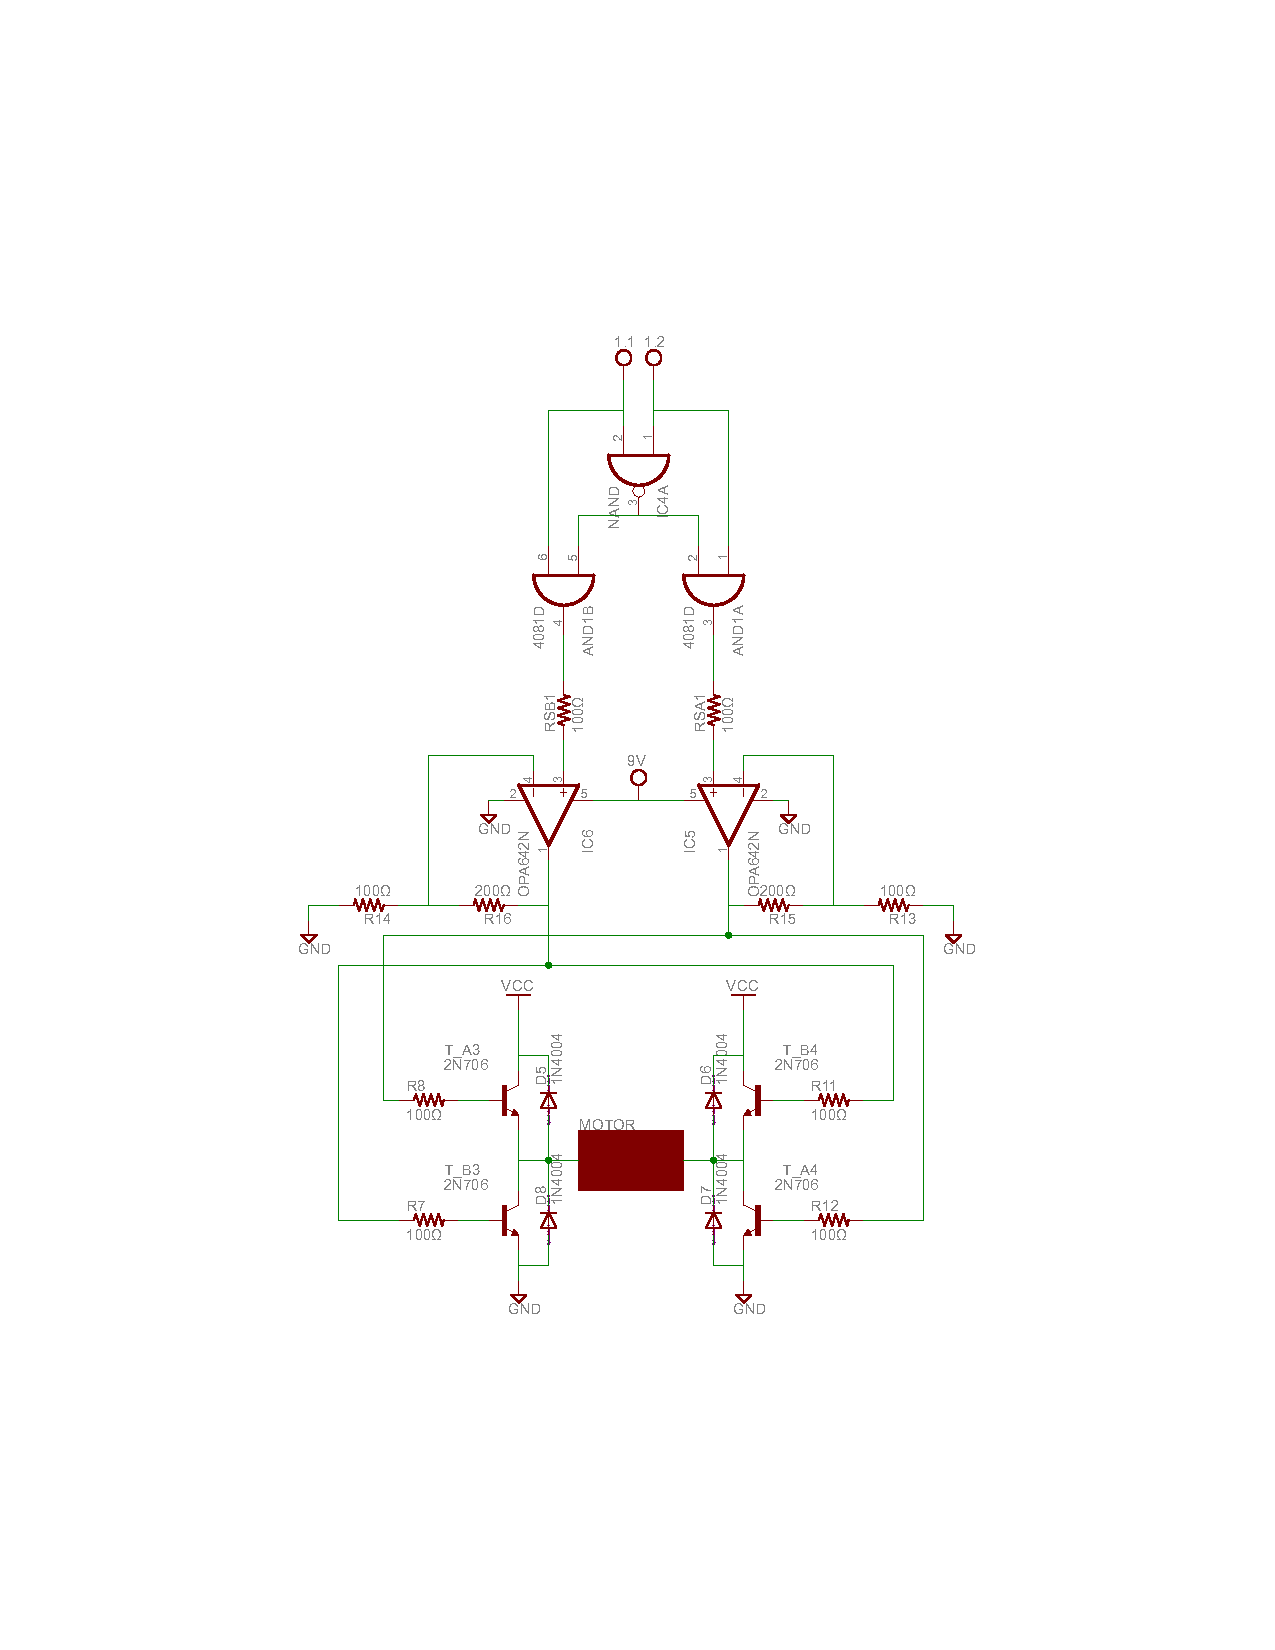
\includegraphics[scale=.8]{report-images/bidirectional-motor-driver}
		\vspace{-4cm}
		\caption{Table Motor Control}
	\end{figure}
	\noindent The motor control consists of an H-bridge (bottom half) for rotation in both directions.  The motor is protected from double-input by logic gates (top half).  The amplifiers are solely for voltage amplification.  The axle of the motor points vertically.
\newpage
	\subsection{Potentiometers}
	\begin{figure}[!ht]
		\centering
		\vspace{-11cm}
		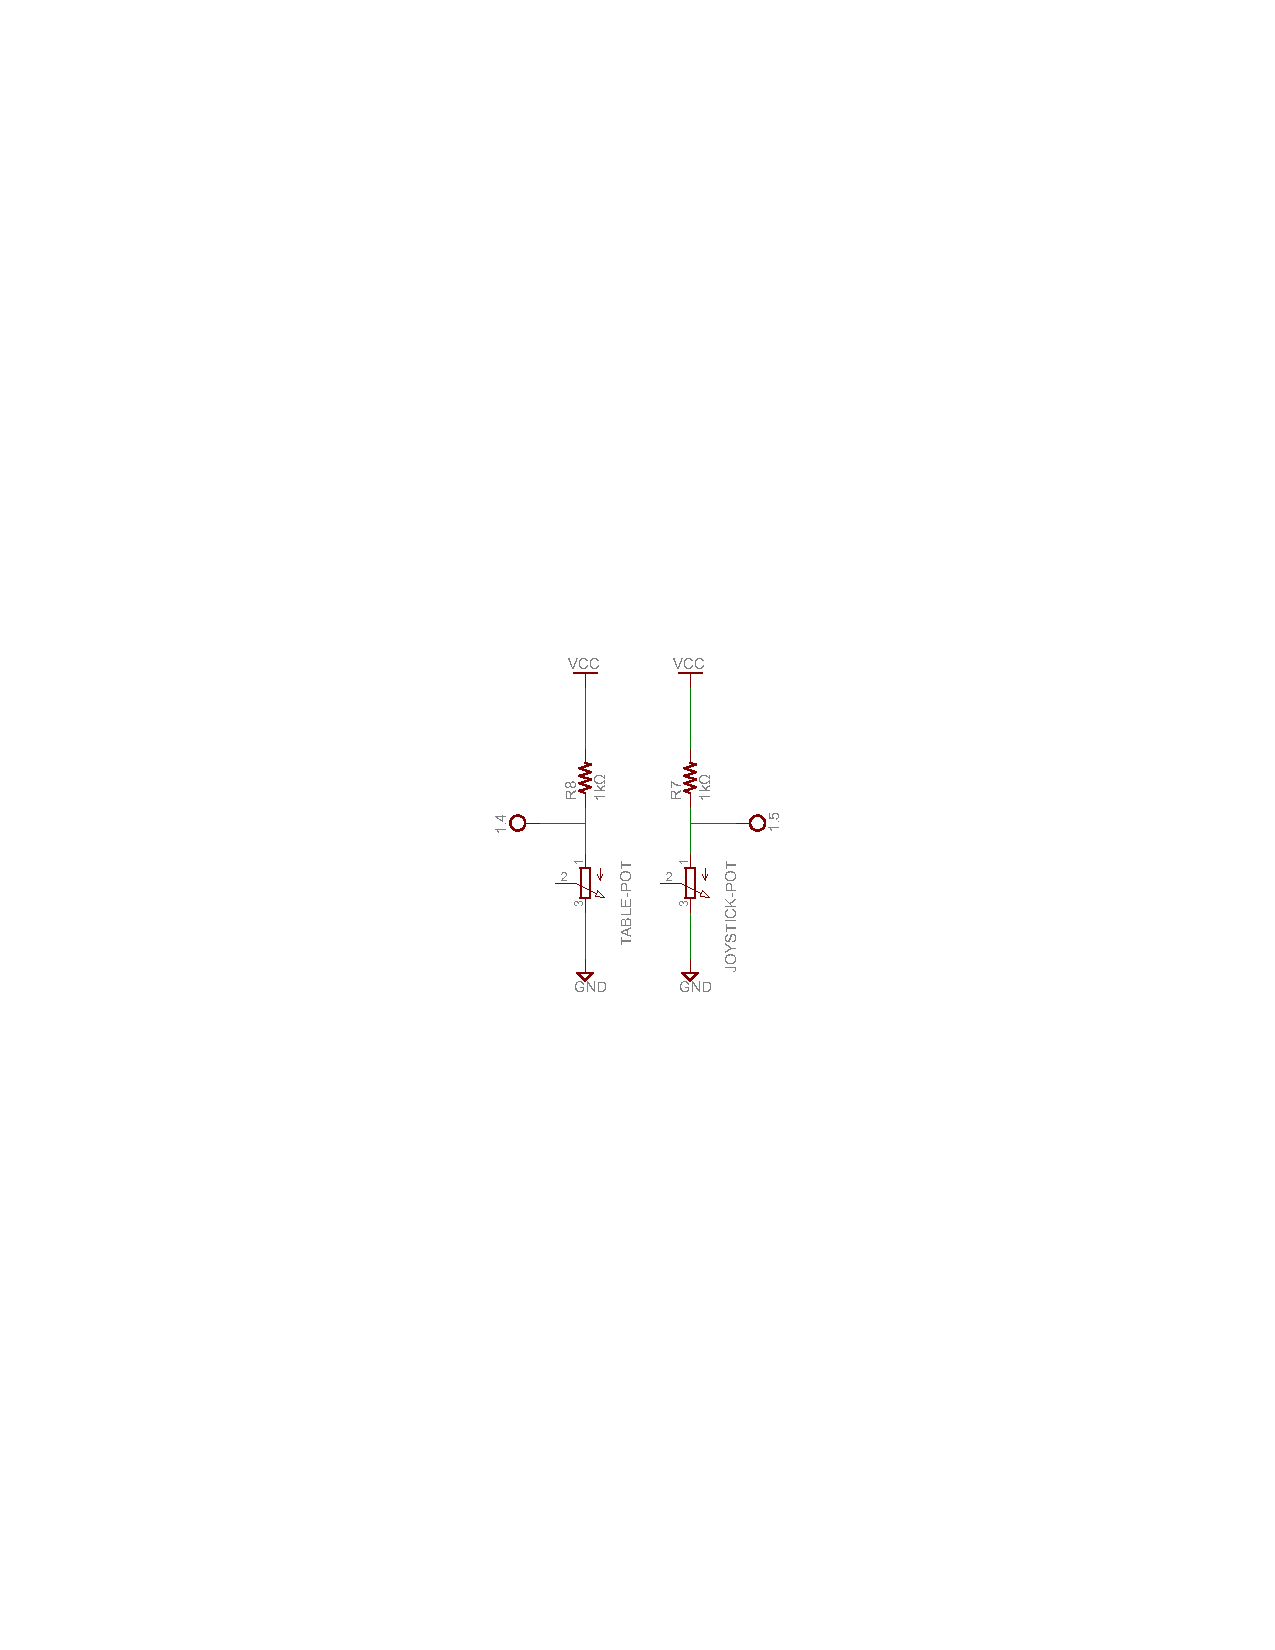
\includegraphics{report-images/potentiometers}
		\vspace{-11cm}
		\caption{Potentiometers}
	\end{figure}
	\noindent The MSP will analogRead the voltage between the resistor and the potentiometer to determine the rotation of the potentiometer.  That in turn will be used as input for PID control to match the two potentiometers.  SOMEONE PLEASE EXPLAIN TO ME WHY \LaTeX IS BEING EVIL AND ADDING RANDOM WHITE SPACE AROUND MY IMAGES
	\subsection{Firing Motor}
	\begin{figure}[!ht]
		\centering
		\vspace{-11cm}
		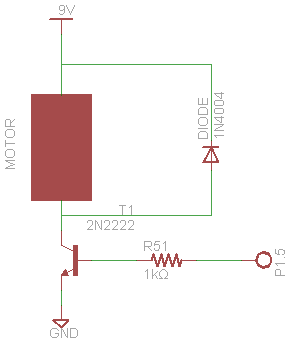
\includegraphics{report-images/firing-motor}
		\vspace{-11.5cm}
		\caption{Firing Motor}
	\end{figure}
\newpage
	\subsection{Firing Button}
	\begin{figure}[!ht]
		\centering
		\vspace{-11cm}
		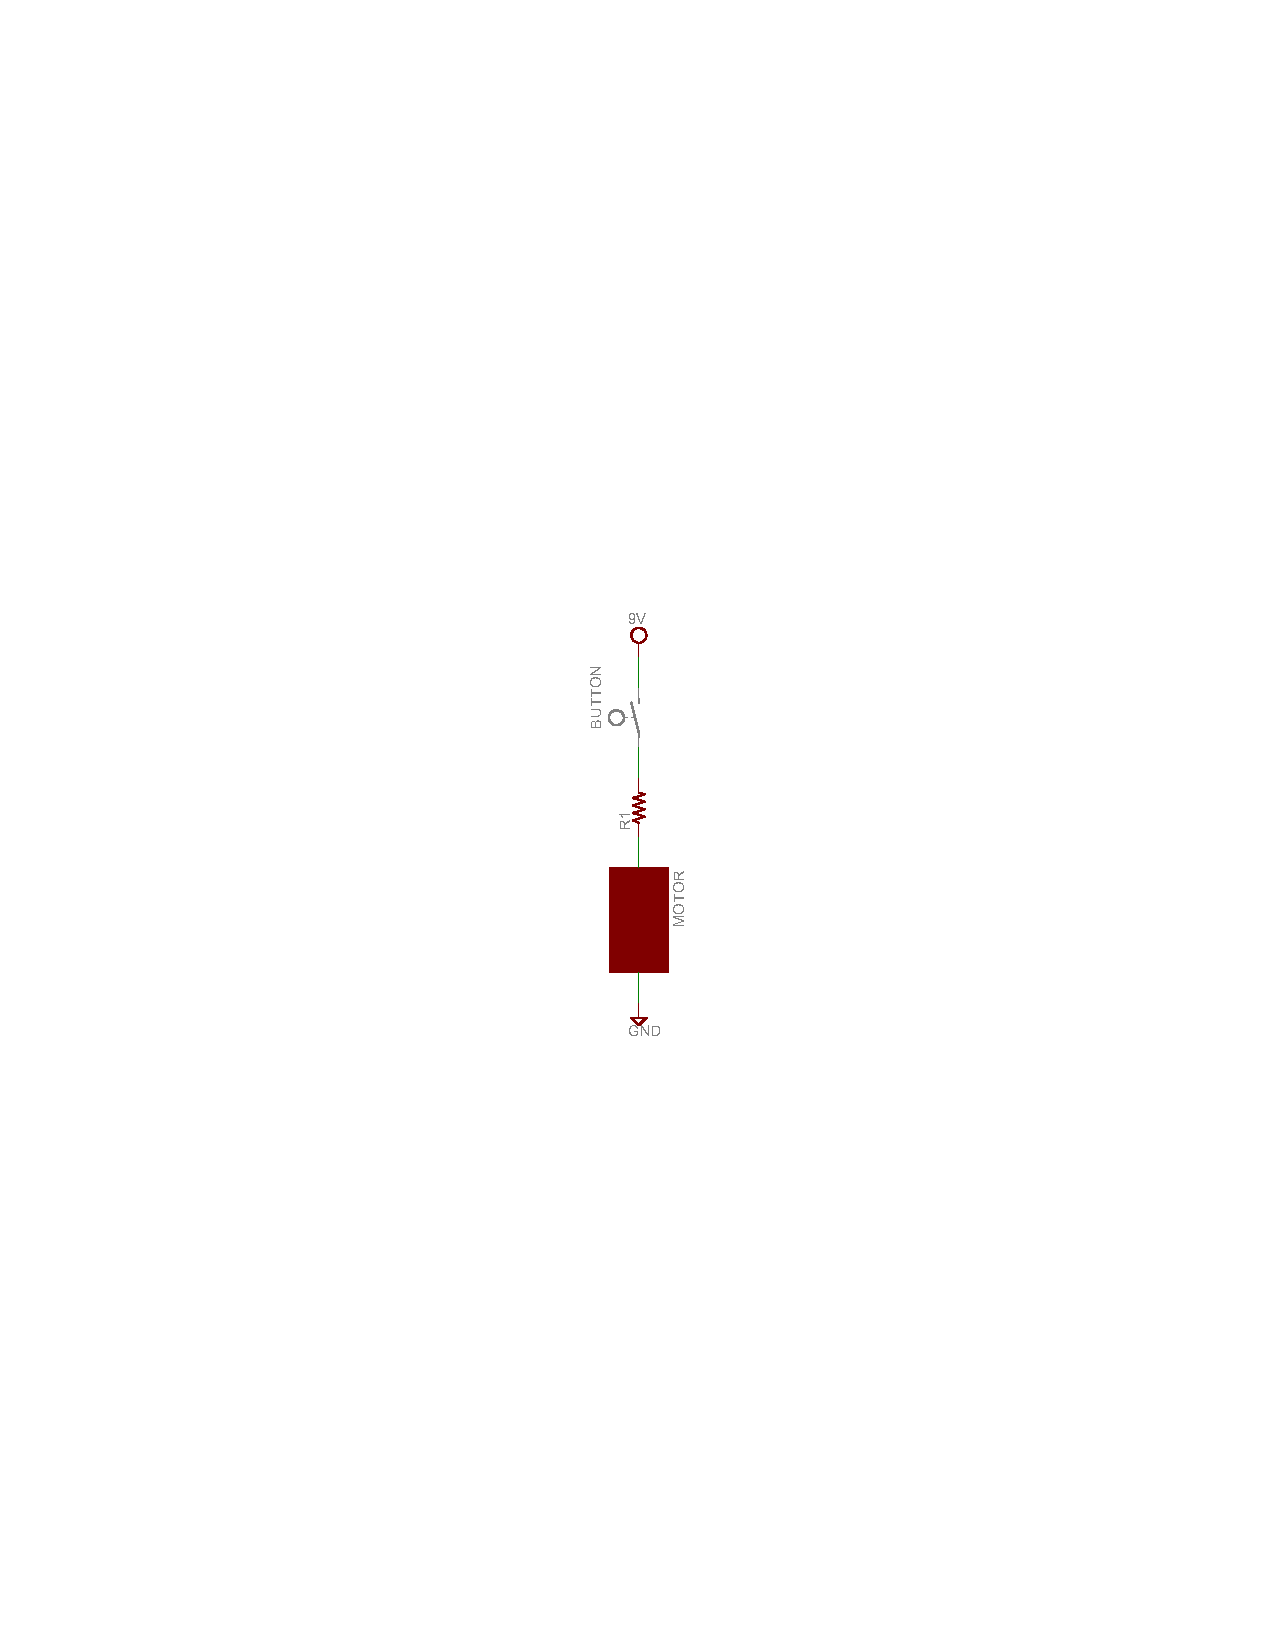
\includegraphics{report-images/firing-button}
		\vspace{-12cm}
		\caption{Firing Button}
	\end{figure}
	\noindent *silent scream of fury at the off-center images*  The MSP will digitalRead the voltage to determine if the button has been pressed.
\newpage
\section{Code}
asdfjkl
% A brief description of extra features (4 lines per feature)
% b. Schematic diagram of the additional analog circuitry
% c. Your MSP430 code with small comment lines explaining the function of each code block.

\end{document}